\section{Napájení}

Jako napájení celého trezoru slouží dvě li-on baterie 18650. Napětí článků však nevyhovuje potřebám trezoru, a~tak je na trezoru lineární 
stabilizátor NCP708, který zajišťuje napětí 3,3~V pro většinu systému. Kromě NPC708 je zde také step-up FP6276, který zajišťuje napájení 5~V 
sloužící primárně ledkám WS2812 a~v~druhá řadě motoru zámku. 

\begin{figure}[htbp]
    \centering
    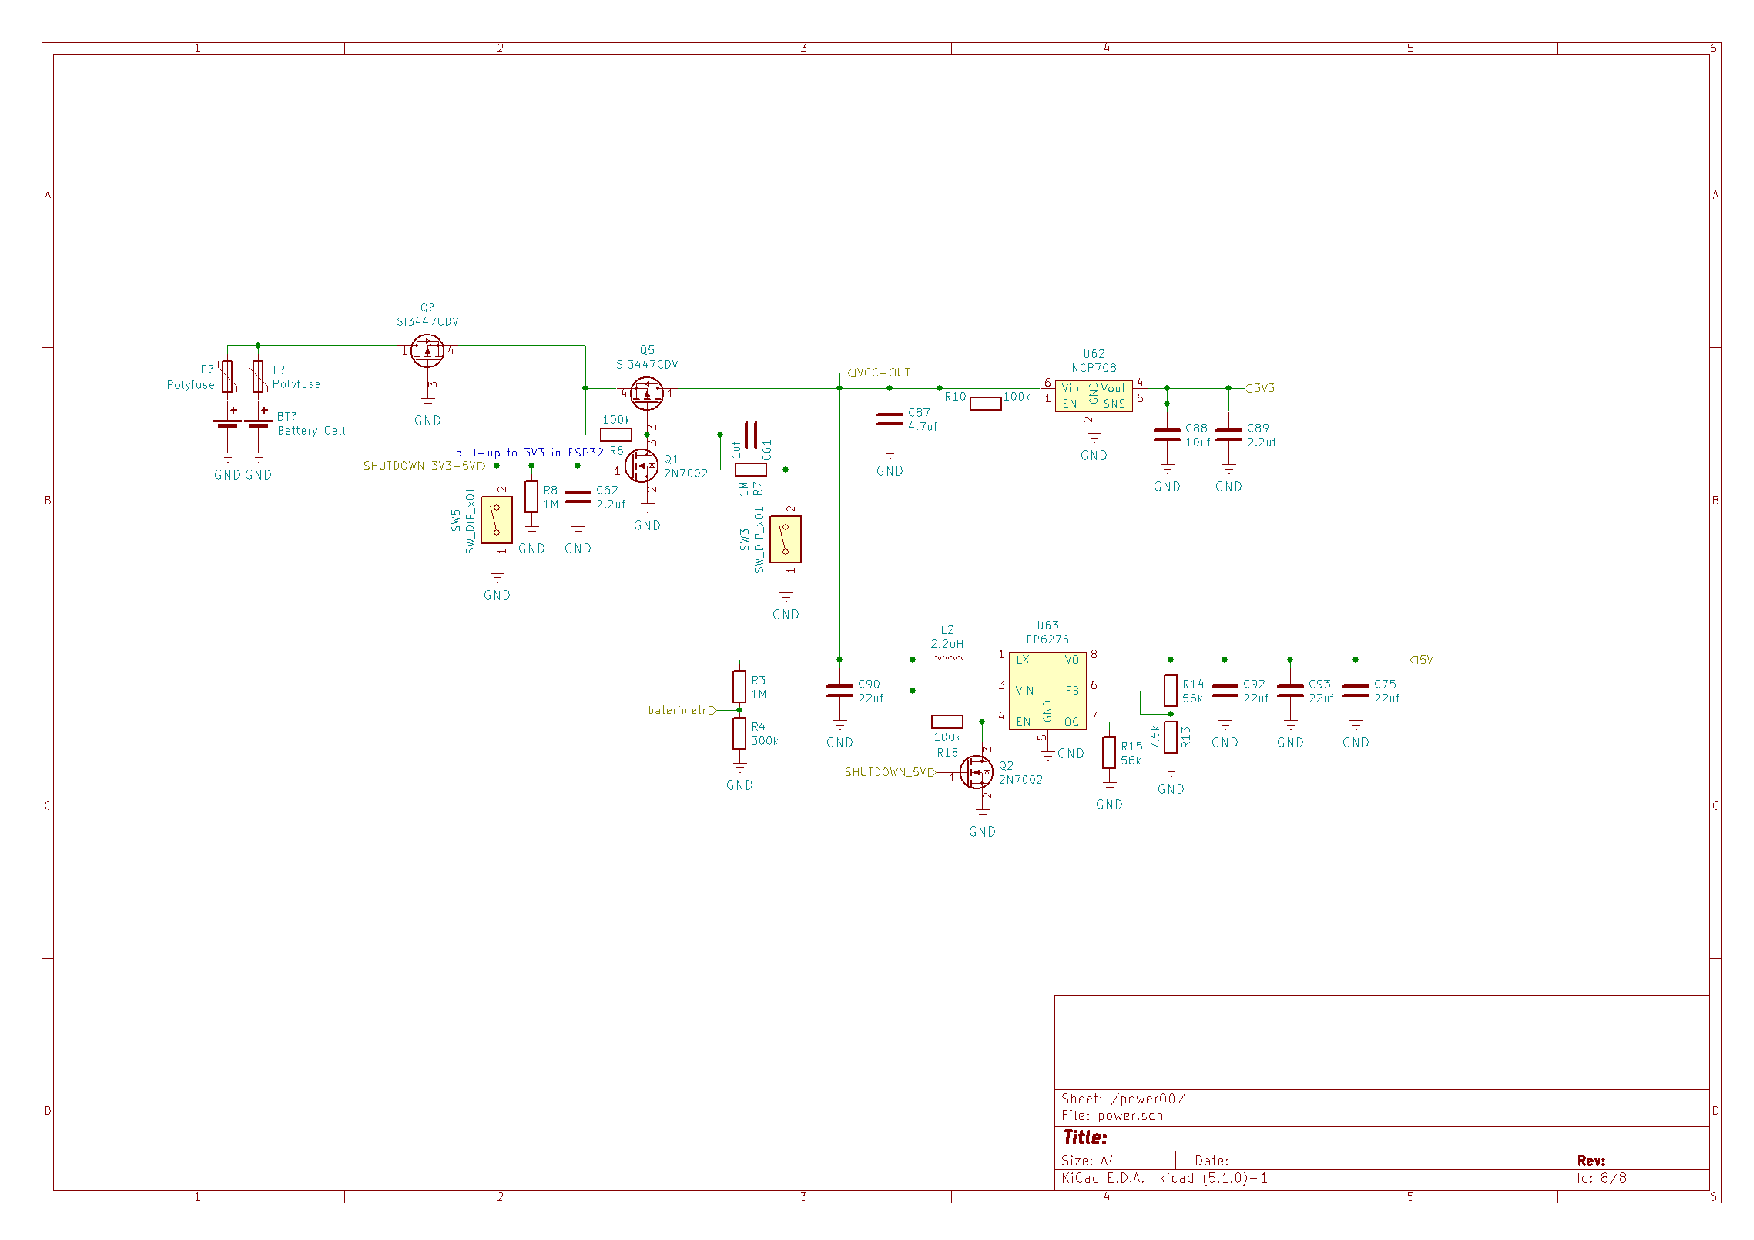
\includegraphics[width=\textwidth]{kapitoly/obrazky/E4/napajeni/zdroj.pdf}
    \caption{zapojení zdroje}
    \label{fig:zdroj}
\end{figure}  %todo do příloh ? 

\newpage

\paragraph*{Zapínání}
\addcontentsline{toc}{paragraph}{Zapínání}

\begin{wrapfigure}{R}{0.5\textwidth}
    \centering
    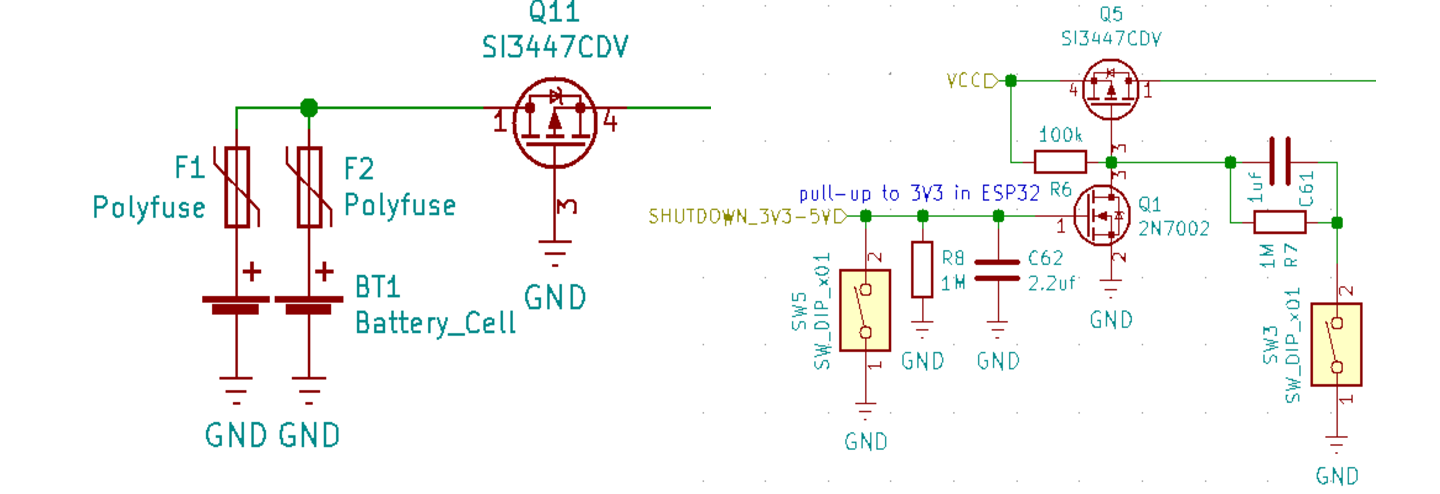
\includegraphics[width=0.55\textwidth]{kapitoly/obrazky/E4/napajeni/ochrana_proti_prepolovani_a_zapinani.png}
    \caption{\label{fig:frog1}Ochrana proti přepólovaní a zapínání}
\end{wrapfigure} %todo oba obrázky bych dal vedle sebe 
Aby se trezor mohl vypnout a~tak šetřit energii, je vybaven obvodem, který to zařizuje.

Při připojení článků se napětí dostane nejprve na polyfuse, %todo česky - vratná pojistka?
které slouží jako ochrana proti nadproudu, například v případě, kdy uživatel připojí dva 
různě nabité články nebo jeden z~nich přepóluje.
Pokud se proud dostane skrz polyfuse, dostane se na tranzistor Q11, skrz který projde, jen pokud jsou články správně otočeny.
Když se napětí dostane přes ochranu proti přepólování, dostane se na S tranzistoru Q5, skrz R6 na D Q1 a~pak skrz R7 na obě strany C61.
Pokud v~takovéto situaci dojde ke~stisku SW3, projde zem skrz C61 na G Q5. V~tu~chvíli se Q5 otevře na dostatečně dlouhou dobu, 
aby naběhla třívoltová větev a~skrz pull-up (na obrázku je jen poznámka, ne reálná součástka) se zvedla napětí na G Q1 na téměř 3,3~V. 
Q1 se tak otevře a~už~trvale připojí GND na G Q5, trezor se tak zapnul. Pokud v takové chvíli procesor stáhne dráhu SHUTDOWN 3V3-5V 
na GND, nebo dojde ke stisku SW5, opět se uzavře Q1 a~skrz R6 projde na G Q5 napětí, které Q5 uzavře a~tak elektroniku opět vypne.

\newpage

\paragraph*{Stabilizátor}
\addcontentsline{toc}{paragraph}{Stabilizátor}

Stabilizátor \href{https://datasheet.lcsc.com/szlcsc/ON-Semicon-ON-NCP708MU330TAG_C183178.pdf}{NCP708} má pin EN, který slouží k~jeho vypínání. 
Pokud je na nem logická 0, je~stabilizátor vypnut a~pokud 1, je zapnut. Vzhledem k~tomu, že v~mém zapojení toto vypínaní nepotřebuji, je pin EN připojen 
přes R10 přímo na napájecí napětí, a~tak je stabilizátor trvale zapnut. Druhý pin, kterým se~NCP708 liší od~jiných stabilizátorů, je~pin~SNS, 
který je vrchní stranou děliče, který určuje výstupní napětí. Vzhledem k~tomu, že je dělič nastaven právě tak, jak potřebuji, nemusím ho~nijak 
upravovat, a~tak~je~SNS napojen přímo na~výstup stabilizátoru. % \newline
Konkrétně NPC708 jsem vybral kvůli malému pádu napětí, který vyžaduje pro svůj provoz, typicky 0,25~V při proudu 1~A. Vzhledem k~tomu, že~na~vstupu 
mám maximálně 4,2~V, tak maximální napěťový pád, který mám k~dispozici je~0,9~V, protože na výstupu požaduji napětí 3,3~V. Navíc musím počítat 
i~s~vybitou baterií, u~které počítám s~napětím 3,5~V. Rád bych počítal s~napětím ještě nižším, ale v~nabídce JLCPCB jsem nenašel stabilizátor 
s~nižším pádem napětí a~zároveň dostatečným proudem. 

\begin{figure}[htbp]
    \centering
    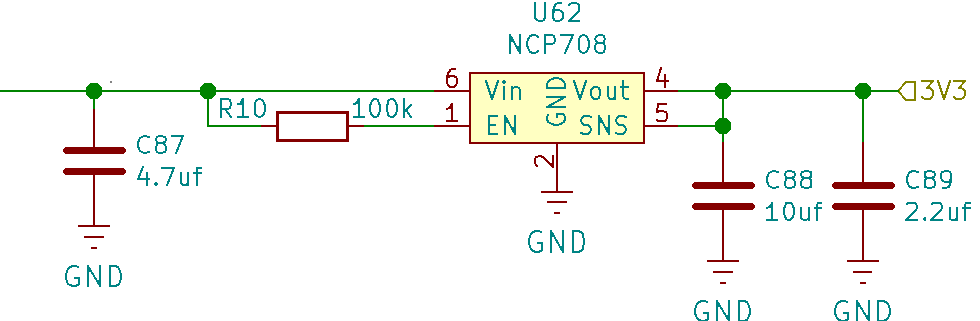
\includegraphics[width=400pt]{kapitoly/obrazky/E4/napajeni/stabilizator.png}
    \caption{Zapojení stabilizátoru}
    \label{fig:E4-stabilizator}
\end{figure}

\paragraph*{Step-up}
\addcontentsline{toc}{paragraph}{Step-up}

\subparagraph*{Step-up vysvětlení funkce}
Zapojení step-upu je~o~něco složitější než stabilizátor, který stačí připojit a funguje. Spínané zdroje využívají ke své funkci cívku, na které
vzniká změna napětí. V případě step-up je to jeho růst. Proud cívkou se nedá okamžitě zastavit a právě to se využívá. 
Když se step-up spustí, připne výstup cívky k~zemi. Ve chvíli, kdy je proud cívkou dostatečný, přepne se výstup cívky na výstup step-upu.
Protože proud cívkou se nedá zastavit a~cívkou už proud teče, zvedne se napětí za cívkou, které začne plnit kondenzátor na výstupu.
Když napětí stoupne nad horní hranici požadovaného napětí, výstup cívky se opět přepne na zem. Ve chvíli, kdy napětí na kondenzátorech opět 
klesne, tím že dodává proud, připojí se cívka. Protože se~na~dobu pádu napětí na~výstupním kondenzátoru připojila cívka na~zem, obnovil 
se~v~ní~proud a~cyklus se tak může opakovat.


\subparagraph*{Step-up zapojení na desce trezoru} 

Pro ovládání spínání step-upu jsem zvolil \href{https://datasheet.lcsc.com/szlcsc/Feeling-Tech-FP6276AXR-G1_C83308.pdf}{FP6276}.
Tento obvod jsem zvolil, protože mi vyhovoval jak po stránce napětí tak po~stránce efektivity a~ceny a~zároveň byl v~nabídce firmy JLCPCB,
u~které jsem desky vyráběl a~osazoval. 
Obvod jsem z~většiny zapojil dle doporučení výrobce, mojí prací bylo vlastně jen správně určit hodnotu 
jednotlivých součástek. Na ovládání pinu EN, který FP6276 vypíná, jsem připojil pull-up k napájení a~pro možnost step-up vypnout tranzistor Q2. 
Pokud procesor stáhne dráhu SHUTDOWN 5V k zemi a~tak přivede na G Q2 zem, Q2 se zavře a~tím se na pin EN přivede skrz R18 napájecí napětí, 
které step-up spustí. Pokud se na G Q2 přivede naopak logická jedna, Q2 se~otevře a~na~EN~se~dostane zem, která naopak provoz step-upu zastaví.

\begin{figure}[htbp]
    \centering
    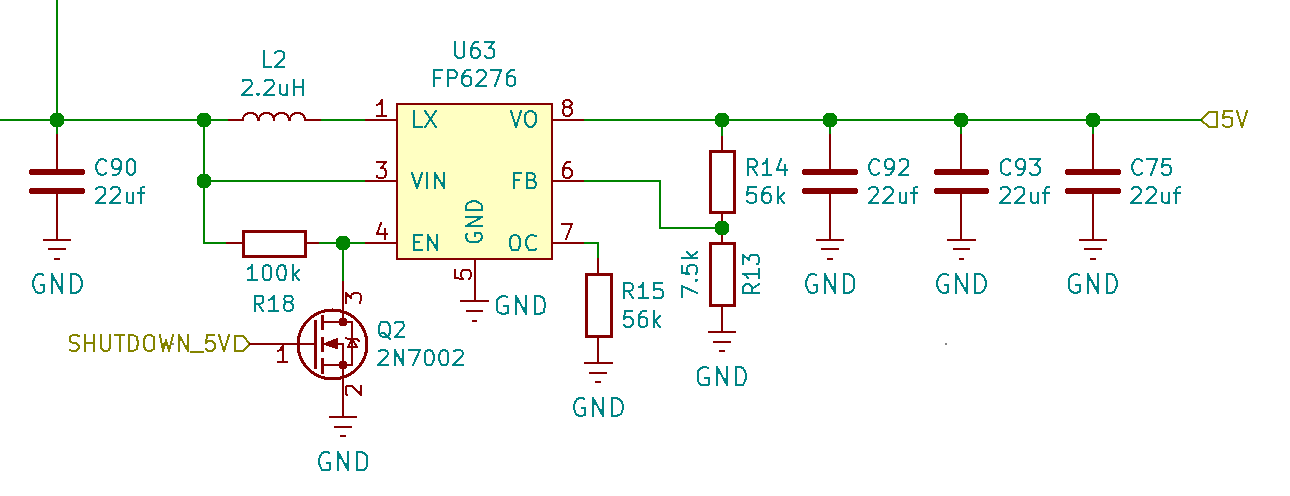
\includegraphics[width=400pt]{kapitoly/obrazky/E4/napajeni/step-up.png}
    \caption{zapojení step-upu}
    \label{fig:E4-step-up}
\end{figure}

\newpage

\paragraph*{Měření napětí baterek}
\addcontentsline{toc}{paragraph}{měření napětí baterek}

\begin{wrapfigure}{R}{0.6\textwidth}
    \centering
    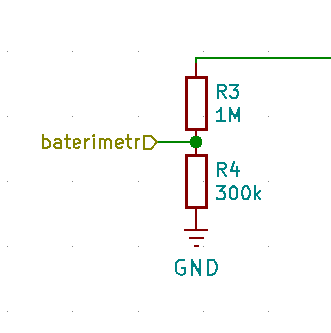
\includegraphics[width=0.6\textwidth]{kapitoly/obrazky/E4/napajeni/delic_baterimetru.png}
    \caption{\label{fig:frog1}}
\end{wrapfigure}

Aby trezor mohl zjistit že má vybité baterie, musí mít možnost jim měřit napětí. ESP32 obsahuje AD převodník takže není problém měřit napětí baterie 
i poměrně přesně, kde však problem nastává, je maximální napětí, které je schopen měřit, a~to 1,1~V. ESP32 sice má možnost připojit k~AD převodníku dělič,
aby se~na~pin dalo přivést napětí až 3,3~V, ale to~pořád není dostatečné, a~také se~tím snižuje přesnost měření. Proto je na desce jednoduchý dělič napětí
složený ze~dvou odporů, jednoho s~hodnotou 1~M$\Omega$ a~druhého 300~k$\Omega$, takže při plně nabitých bateriích bude na výstupu děliče 0,97~V. %todo kolik je tam těch baterek

\newpage